% Author: Izaak Neutelings (Februari, 2020)
% http://texample.net/tikz/examples/tag/circuitikz/
% http://texample.net/tikz/examples/circuitikz/
% https://www.overleaf.com/learn/latex/CircuiTikz_package
% http://texdoc.net/texmf-dist/doc/latex/circuitikz/circuitikzmanual.pdf
% http://repositorios.cpai.unb.br/ctan/graphics/pgf/contrib/circuitikz/circuitikzmanual.pdf
\documentclass[border=3pt,tikz]{standalone}
\usepackage{amsmath} % for \dfrac
\usepackage{physics}
\usepackage{tikz,pgfplots}
\usepackage[siunitx,european]{circuitikz} %[symbols]
\usepackage[outline]{contour} % glow around text
\usetikzlibrary{arrows}
\usetikzlibrary{decorations.markings}
\tikzset{>=latex} % for LaTeX arrow head
\usepackage{xcolor}
\definecolor{r1}{HTML}{FF8674}
\definecolor{b1}{HTML}{17ABDD}
\definecolor{p1}{HTML}{D4B6D6}
\definecolor{g1}{HTML}{70E2CB}
\definecolor{o1}{HTML}{DFA743}


\colorlet{Ccol}{orange!90!black}
\colorlet{pluscol}{red!60!black}
\colorlet{minuscol}{blue!60!black}

\usepackage{BOONDOX-cal} %使用花体emf
\newcommand\EMF{\mathcal{E}} %\varepsilon}
%\tikzstyle{charged}=[top color=blue!20,bottom color=blue!40,shading angle=10]
\contourlength{1.5pt}
\tikzstyle{EMF}=[battery1,l=$\EMF$]
\tikzstyle{internal R}=[R,color=b1,b1,l=$r$,/tikz/circuitikz/bipoles/length=30pt]
\tikzstyle{loop}=[->,red!90!black!25]
\tikzstyle{loop label}=[r1,fill=white,scale=0.8,inner sep=1]
\tikzstyle{thick R}=[R,color=b1,thick,b1,l=$R$]
%\tikzset{
%  loop/.style={thick,red!80!black!30,decoration={markings,
%               mark=at position #1 with {\arrow{latex}}},
%               postaction={decorate}},
%  loop/.default=0.6}


\newcommand{\myvoltmeter}[2] 
{  % #1 = name , #2 = rotation angle
  \begin{scope}[transform shape,rotate=#2]
  \draw[thick] (#1)node(){$\mathbf V$} circle (11pt);
  \draw[rotate=45,-latex] (#1)  +(-17pt,0) --+(17pt,0);
  \end{scope}
}


\begin{document}


% RESISTOR without battery
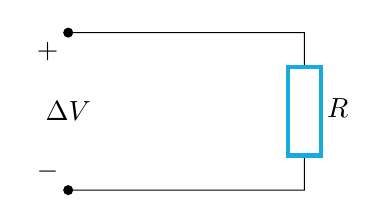
\begin{tikzpicture}
  \draw (0,2) to [short,*-] (3,2) to[R,color=b1,thick,l=$R$] (3,0) to [short,-*] (0,0);
  \node[below left] at (0,2) {$+$};
  \node[above left] at (0,0) {$-$};
  \node at (0,1) {$\Delta V$};
\end{tikzpicture}


% RESISTOR with battery and arrow
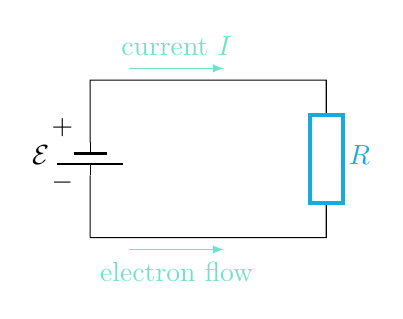
\begin{tikzpicture}
  \draw (0,0) to[EMF] (0,2) -- (3,2)
              to[thick R] (3,0) -- (0,0);
  \node at (-0.35,0.7) {$-$};
  \node at (-0.35,1.4) {$+$};
  \draw[->,g1] (0.5, 2.15) --++ (1.2,0) node[midway,above=1] {current $I$};
  \draw[->,g1] (0.5,-0.15) --++ (1.2,0) node[midway,below=1] {electron flow};
\end{tikzpicture}


% RESISTOR with battery and arc arrow
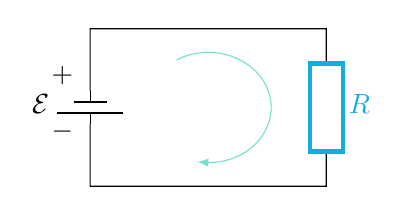
\begin{tikzpicture}
  \def\ang{120}
  \def\a{0.8}
  \def\b{0.7}
  \draw (0,0) to[EMF] (0,2) -- (3,2)
              to[thick R] (3,0) -- (0,0);
  \node at (-0.35,0.7) {$-$};
  \node at (-0.35,1.4) {$+$};
  \draw[->,g1] ({1.5+\a*cos(\ang)},{1+\b*sin(\ang)}) arc (120:-100:{\a} and {\b});
\end{tikzpicture}


% RESISTOR with EMF + internal resistance
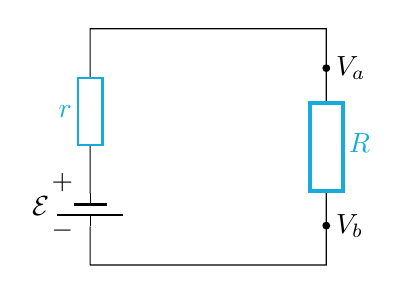
\begin{tikzpicture}
  \draw (0,0) to[EMF] (0,1.4)
              to[internal R] (0,2.5) -- (0,3) --++ (3,0)
              to[thick R] ++(0,-3) -- (0,0);
  %\draw (3,2.5) --++ (0.6,0) to[voltmeter,color=white,name=M] ++(0,-2) --++ (-0.6,0);
  %\myvoltmeter{M}{0} % rotate
  \fill[black] (3,2.5) circle (0.05) node[right] {$V_a$};
  \fill[black] (3,0.5) circle (0.05) node[right] {$V_b$};
  \node at (-0.35,0.44) {$-$};
  \node at (-0.35,1.05) {$+$};
\end{tikzpicture}


% RESISTOR with EMF + internal resistance
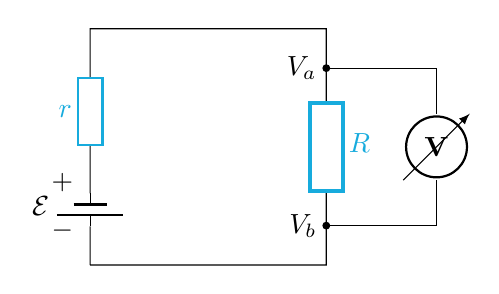
\begin{tikzpicture}
  \draw (0,0) to[EMF] (0,1.4)
              to[internal R] (0,2.5) -- (0,3) --++ (3,0)
              to[thick R] ++(0,-3) -- (0,0);
  \draw (3,2.5) --++ (1.4,0) to[voltmeter,color=white,name=M] ++(0,-2) --++ (-1.4,0);
  \myvoltmeter{M}{0} % rotate
  \fill[black] (3,2.5) circle (0.05) node[left] {$V_a$};
  \fill[black] (3,0.5) circle (0.05) node[left] {$V_b$};
  \node at (-0.35,0.44) {$-$};
  \node at (-0.35,1.05) {$+$};
\end{tikzpicture}


%% RESISTOR with EMF + internal resistance
%\begin{tikzpicture}
%  \draw (0,0) to[EMF] (0,1.4)
%              to[internal R] (0,2.5) -- (0,3) --++ (3,0)
%              --++ (0,-0.5) coordinate (T) --++ (-0.9,0)
%              to[thick R] ++(0,-2) --++ (0.9,0) |- (0,0)
%        (T) --++ (0.9,0) to[voltmeter,color=white,name=M] ++(0,-2) --++ (-0.9,0); %,l=$R$
%  \myvoltmeter{M}{0} % rotate
%  \node at (-0.35,0.44) {$-$};
%  \node at (-0.35,1.05) {$+$};
%\end{tikzpicture}
%
%
%% RESISTOR with EMF + internal resistance + boxes
%\begin{tikzpicture}
%  \draw (0,0) to[EMF] (0,1.4)
%              to[internal R] (0,2.5) -- (0,3) --++ (3,0)
%              --++ (0,-0.5) coordinate (T) --++ (-0.9,0)
%              to[thick R] ++(0,-2) --++ (0.9,0) |- (0,0)
%        (T) --++ (0.9,0) to[voltmeter,color=white,name=M] ++(0,-2) --++ (-0.9,0); %,l=$R$
%  \myvoltmeter{M}{0} % rotate
%  \node at (-0.35,0.44) {$-$};
%  \node at (-0.35,1.05) {$+$};
%  \draw[dashed,very thin] (-0.9,0.3) rectangle (0.8,2.7);
%  \draw[dashed,very thin] ( 1.6,0.3) rectangle (4.5,2.7);
%\end{tikzpicture}


% RESISTOR with EMF + AMPEREMETER + VOLTMETER
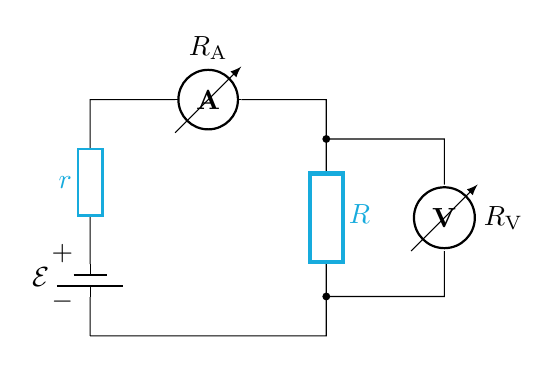
\begin{tikzpicture}
  \draw (0,0) to[EMF] (0,1.4)
              to[internal R] (0,2.5) -- (0,3) to[ammeter] ++(3,0)
              to[thick R] ++(0,-3) -- (0,0);
  \draw (3,2.5) --++ (1.5,0) to[voltmeter,color=white,name=M] ++(0,-2.0) --++ (-1.5,0);
  \fill[black] (3,2.5) circle (0.05);
  \fill[black] (3,0.5) circle (0.05);
  \myvoltmeter{M}{0} % rotate
  \node at (-0.35,0.44) {$-$};
  \node at (-0.35,1.05) {$+$};
  \node[] at (1.5,3.65) {$R_\mathrm{A}$};
  \node[] at (5.25,1.5) {$R_\mathrm{V}$};
\end{tikzpicture}


% KIRCHHOFF's RULE 1
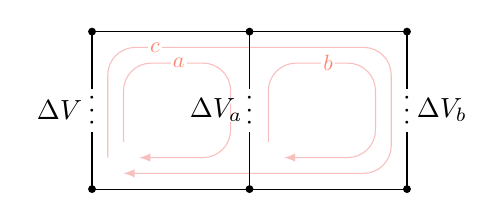
\begin{tikzpicture}
  \def\a{0.2}
  \def\b{0.4}
  \def\H{2}
  \def\W{2}
  \draw[rounded corners=10,loop] (\a,2*\a) |- (2*\W-\a,\H-\a) |- (2*\a,\a);
  \draw[rounded corners=10,loop] (\b,\b+\a) |- (\W-.6*\b,\H-\b) |- (\b+\a,\b);
  \draw[rounded corners=10,loop] (\W+.6*\b,\b+\a) |- (2*\W-\b,\H-\b) |- (\W+.6*\b+\a,\b);
  \fill[black] (0,\H) circle (0.05); %node[above] {$V_i$};
  \fill[black] (0,0) circle (0.05); %node[below] {$V_f$};
  \fill[black] (\W,\H) circle (0.05); %node[above] {$V_{1a}$};
  \fill[black] (\W,0) circle (0.05); %node[below] {$V_{1b}$};
  \fill[black] (2*\W,\H) circle (0.05); %node[above] {$V_{2a}$};
  \fill[black] (2*\W,0) circle (0.05); %node[below] {$V_{2b}$};
  \draw ( 0,0) |- ++(\W,\H) |- cycle;
  \draw (\W,0) -| ++(\W,\H) --++ (-2,0);
  \node[fill=white,rotate=90,inner sep=2] at (0,\H/2) {$.\,.\,.$};
  \node[fill=white,rotate=90,inner sep=2] at (\W,\H/2) {$.\,.\,.$};
  \node[fill=white,rotate=90,inner sep=2] at (2*\W,\H/2) {$.\,.\,.$};
  \node[left] at (0,\H/2) {$\Delta V$};
  \node[left=-1] at (\W,\H/2) {\contour{white}{$\Delta V_a$}};
  \node[right] at (2*\W,\H/2) {$\Delta V_b$};
  \node[loop label] at (0.40*\W,0.90*\H) {$c$};
  \node[loop label] at (0.55*\W,0.80*\H) {$a$};
  \node[loop label] at (1.50*\W,0.80*\H) {$b$};
\end{tikzpicture}


% KIRCHHOFF's RULE 2
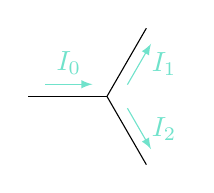
\begin{tikzpicture}
  \def\r{0.6}
  \def\R{1}
  \coordinate (O) at (0,0);
  \draw (O) --++ (180:\R);
  \draw (O) --++ (60:\R);
  \draw (O) --++ (-60:\R);
  \draw[<-,g1] (O)++(140:0.4*\r) --++ (180:\r) node[midway,above] {$I_0$};
  \draw[->,g1] (O)++( 30:0.5*\r) --++ ( 60:\r) node[midway,right=1] {$I_1$};
  \draw[->,g1] (O)++(-30:0.5*\r) --++ (-60:\r) node[midway,right=1] {$I_2$};
\end{tikzpicture}


% RESISTOR in series
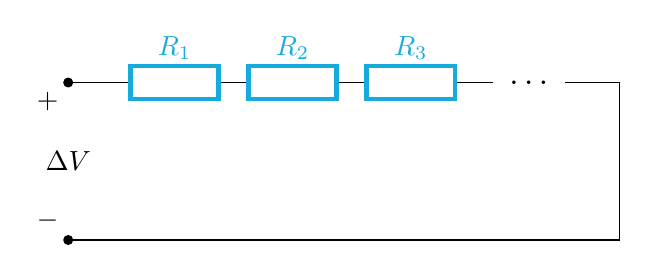
\begin{tikzpicture}
  \draw (0,2) to [short,*-] (0.6,2)
              to[thick R,l=$R_1$] ++(1.5,0)
              to[thick R,l=$R_2$] ++(1.5,0)
              to[thick R,l=$R_3$] ++(1.5,0)
              -- ++(1.5,0) node[midway,fill=white,inner sep=5,scale=1.2] {$.\,.\,.$}
              -- (7,2) -- (7,0) to[short,-*] (0,0);
  \node at (0,1) {$\Delta V$};
  \node[below left] at (0,2) {$+$};
  \node[above left] at (0,0) {$-$};
\end{tikzpicture}


% RESISTOR in parallel
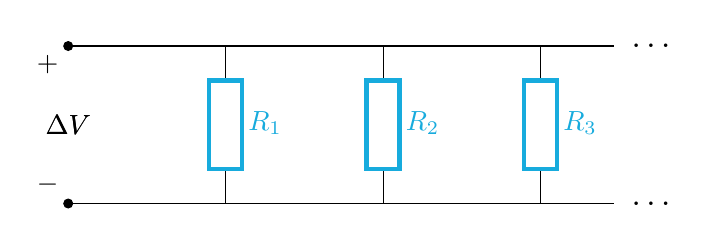
\begin{tikzpicture}
  \node[fill=white,inner sep=5,scale=1.2] (ET) at (7.4,2) {$.\,.\,.$};
  \node[fill=white,inner sep=5,scale=1.2] (EB) at (7.4,0) {$.\,.\,.$};
  \node at (0,1) {$\Delta V$};
  \draw (0,2) to[short,*-] (2,2) to[thick R,l=$R_1$] (2,0) to[short,-*] (0,0);
  \draw (2,2) -- (4,2) to[thick R,l=$R_2$] (4,0) -- (2,0);
  \draw (4,2) -- (6,2) to[thick R,l=$R_3$] (6,0) -- (4,0);
  \draw (6,2) -- (ET.180);
  \draw (6,0) -- (EB.180);
  \node at (0,1) {$\Delta V$};
  \node[below left] at (0,2) {$+$};
  \node[above left] at (0,0) {$-$};
\end{tikzpicture}


% RESISTOR in series - zoomed in
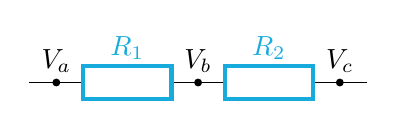
\begin{tikzpicture}
  \def\a{1.8}
  \def\b{0.35}
  \draw (-\b,0) -- (0,0) to[thick R,l=$R_1$] (\a,0) to[thick R,l=$R_2$] (2*\a,0) --++ (\b,0);
  \fill (0,0) circle (0.05) node[above] {$V_a$};
  \fill (\a,0) circle (0.05) node[above] {$V_b$};
  \fill (2*\a,0) circle (0.05) node[above] {$V_c$};
\end{tikzpicture}


% RESISTOR in parallel - R1, R2
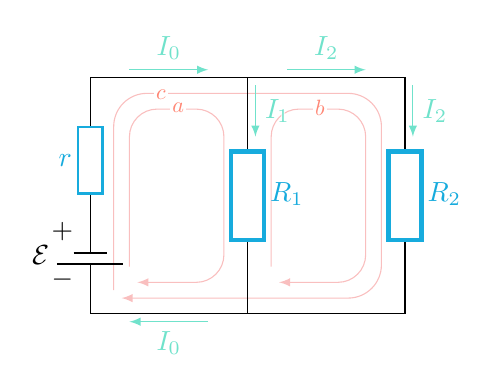
\begin{tikzpicture}
  \draw[rounded corners=12,loop] (0.3,0.3) |- (3.7,2.8) |- (0.4,0.2);
  \draw[rounded corners=10,loop] (0.5,0.6) |- (1.7,2.6) |- (0.6,0.4);
  \draw[rounded corners=10,loop] (2.3,0.6) |- (3.5,2.6) |- (2.4,0.4);
  \draw (0,0) to[EMF] (0,1.4)
              to[internal R] (0,2.5)
              -- (0,3) coordinate (I0) --++ (2,0) coordinate (I1)
              to[thick R,l=$R_1$] (2,0) coordinate (IF) -- (0,0);
  \draw (2,3) --++ (2,0) coordinate (I2)
              to[thick R,l=$R_2$] (4,0) -- (0,0);
  \node at (-0.35,0.44) {$-$};
  \node at (-0.35,1.05) {$+$};
  \draw[->,g1] (I0)++(0.5, 0.1) --++ (1,0) node[midway,above] {$I_0$};
  \draw[->,g1] (I1)++(0.1,-0.1) --++ (0,-0.65) node[midway,right] {\contour{white}{$I_1$}};
  \draw[->,g1] (I1)++(0.5, 0.1) --++ (1,0) node[midway,above] {$I_2$};
  \draw[->,g1] (I2)++(0.1,-0.1) --++ (0,-0.65) node[midway,right] {$I_2$};
  \draw[->,g1] (IF)++(-0.5,-0.1) --++ (-1,0) node[midway,below] {$I_0$};
  \node[loop label] at (0.90,2.78) {$c$};
  \node[loop label] at (1.12,2.62) {$a$};
  \node[loop label] at (2.92,2.62) {$b$};
\end{tikzpicture}


% RESISTOR in parallel - R12
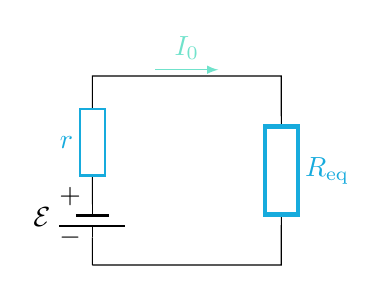
\begin{tikzpicture}[scale=0.8]
  \draw (0,0) to[EMF] (0,1.4)
              to[internal R] (0,2.5) -- (0,3) coordinate (I0) --++ (3,0)
              to[thick R,l=$R_\mathrm{eq}$] (3,0) -- (0,0); %R_{12}
  \node at (-0.35,0.43) {$-$};
  \node at (-0.35,1.08) {$+$};
  \draw[->,g1] (I0)++(1.0, 0.1) --++ (1,0) node[midway,above] {$I_0$};
\end{tikzpicture}


% RESISTOR in parallel - R12r
\begin{tikzpicture}[scale=0.7]
  \draw (0,0) to[EMF] (0,3) --++ (3,0)
              to[thick R,l=$R$] (3,0) -- (0,0); %_{12r}
  \node at (-0.35,1.15) {$-$};
  \node at (-0.35,1.90) {$+$};
  \draw[->,g1] (I0)++(1.0, 0.1) --++ (1,0) node[midway,above] {$I_0$};
\end{tikzpicture}


\end{document}